\section*{Author Response {\color{red}(Supplement)}}
\label{section:author-response}
\addcontentsline{toc}{section}{Author Response (Supplement)}

We sincerely thank Reviewer 4E4z (\textcolor{green}{$@$R1}), 6KzT (\textcolor{red}{$@$R2}), 
JFL4 (\textcolor{blue}{$@$R3}), and V1rg (\textcolor{orange}{$@$R4}) for their thoughtful feedback 
and for highlighting the strengths of our work in \textit{temporal consistency} 
(\textcolor{green}{$@$R1}\textcolor{red}{$@$R2}\textcolor{blue}{$@$R3}\textcolor{orange}{$@$R4}), 
\textit{experimental validation} (\textcolor{red}{$@$R2}\textcolor{blue}{$@$R3}\textcolor{orange}{$@$R4}), 
and \textit{novelty} (\textcolor{green}{$@$R1}\textcolor{red}{$@$R2}\textcolor{blue}{$@$R3}\textcolor{orange}{$@$R4}).

As noted in our original submission, \textbf{we have provided a project page with extensive video results included in the supplementary materials. 
Please ensure that the entire supplementary archive is fully uncompressed before opening the webpage.} 
The page has been successfully tested on both macOS and Windows~10 systems.

%We will also release our implementation to further enhance transparency and reproducibility.

We will make further revisions to the main paper based on the reviewers' feedback. We appreciate your constructive comments and look forward to any additional suggestions.





\subsection{Comparison with Other Baselines \textcolor{green}{$@$R1}}

We have added InstaDrive \cite{yang25instadrive} as a baseline in Tab.~\ref{tab:fvd} and Tab.~\ref{tab:tracking}. Across all metrics, including FID, FVD, and tracking evaluations, InstaDrive consistently performs worse than our method, validating the effectiveness of our approach.

InstaDrive uses an Instance Flow Guider Module to encode trajectory information into an RGB motion map via an optical-flow–like process. This method incurs a high computational cost and may suffer from information loss due to clipping when motion exceeds thresholds. 

In contrast, our Trajectory Mask constructs an instance-specific attention corridor with 3D-tracked trajectories, enabling feature propagation without quantization loss, ensuring better instance-level temporal consistency.



\subsection{Challenges for Occlusion in Non-Continuous Trajectory \textcolor{green}{$@$R1} \textcolor{orange}{$@$R4}}

\textbf{Method:} Instance-Masked Attention ensures consistent instance identity even when objects are occluded and reappear, the principle is demonstrated in Fig.~\ref{fig: main} (c). 
When an object (e.g., object 1) becomes occluded at frame $t+1$ and reappears at frame $t+2$, the Indicator function $I(v_k)$ tracks the object's presence across frames. At frame $t$, $1 \in I(v_0)$ when the object is visible. At frame $t+1$, the object is occluded, and at frame $t+2$, $1 \in I(v_4)$ when the object reappears.
To ensure correct feature propagation, we set $M(0, 4) = 0$ in the Instance Trajectory Mask, allowing attention between token $v_0$ and $v_4$. This enables the reliable propagation of instance-specific features across their trajectory, even after occlusion.

\textbf{Qualitative results} demonstrating our method’s handling of non-continuous trajectories are shown in Fig.~\ref{fig:Non-Continuous}, where the car maintains its identity despite temporary occlusion.

\begin{figure}[ht]
\centering
\includegraphics[width=0.5\linewidth]{figures/continuous.pdf} 
\caption{Challenges for Non-Continuous Trajectory. 
\textbf{(a)} Without the Trajectory Mask in the Instance-Masked Attention module, the car is occluded and reappears, but its color changes from white to black.
\textbf{(b)} With our Instance-Masked Attention, the car preserves its identity and features even after occlusion and reappearance.}
\label{fig:Non-Continuous}
\vspace{-0.5cm}
\end{figure}



%%%%%%%%%%%%%%%%%%%%%%%%%%%%%%%%%%%%%%%%%%%%%%%%%%%%%%%%%%%%%%


\subsection{Novelty Compared to Prior Work\textcolor{red}{$@$R2}}
We appreciate the reviewer’s comments and clarify that the core novelty of \titleDef~ lies in introducing trajectory-grounded, instance-aware attention and supervision mechanisms that directly address fine-grained identity consistency in long-horizon driving video generation—a problem not tackled by prior works.

\textbf{Masked Attention Novelty. }
Our instance-masked attention has two innovations that differ fundamentally from Mask2Former \cite{cheng2022maskedattentionmasktransformeruniversal}.
(i) Our \emph{Trajectory Mask} establishes an instance-specific attention corridor across frames using 3D-tracked trajectories.
This enables tokens belonging to the same object to exchange information over time, 
thereby preserving semantic identity across the full video sequence. 
Such \textit{temporally linked attention} does not exist in Mask2Former or other masked-attention architectures, which 
perform mask-guided attention \textit{within a single frame} for segmentation, without any mechanism for temporal identity modeling or cross-frame feature propagation. 
%
(ii) Our masks are deterministically \textit{constructed from 3D-tracked trajectories}, explicitly controlling which spatial–temporal token interactions are permitted.
In contrast, spatial masks in Mask2Former \textit{originate from per-frame predictions} and are not used to regulate cross-frame feature flow or identity binding. 

%our \emph{Identity Mask} introduces global instance condition tokens that persist across time, acting as identity anchors for all frames.
%This facilitates long-range propagation of instance-level semantics (e.g., category, size, tracking ID) and enforces consistent visual behavior. 





\textbf{Masked Loss Novelty.}
The proposed \emph{Instance-Masked Loss} serves a fundamentally different purpose from Focal Loss \cite{lin2018focallossdenseobject}.  
Focal Loss is \emph{sample-aware}: It reweights individual samples based on prediction confidence to mitigate class imbalance in static image tasks.  
In contrast, our loss is \emph{pixel-aware} and leverages 3D-projected instance regions to 
construct instance masks, ensuring that foreground objects receive sufficient supervision across all frames.
This mechanism directly supports the goal of improving instance-level temporal consistency, which is not addressed by Focal Loss or related formulations.
%counteract a different problem unique to diffusion-based driving video generation—gradient dilution, where large background areas dominate the denoising loss and cause small moving objects to fade over time.

%Our loss does not depend on confidence scores, class imbalance, or per-sample weighting. 

%Instead, it is tightly coupled with the temporally consistent instance masks derived from 3D annotations, ensuring that foreground objects receive sufficient supervision across all frames. 




\textbf{Pipeline Novelty.}
Our method targets a different problem compared to CineMaster~\cite{wang2025cinemaster3dawarecontrollableframework}.  
CineMaster focuses on \emph{controllable video generation} to regulate \textit{per-frame} layout. 
It does not preserve instance identities \textit{across frames}.
In contrast, ConsisDrive addresses \emph{instance-level temporal consistency}, a key failure in driving world models. 
Our method introduces identity- and trajectory-aware masks \emph{inside the diffusion transformer’s attention blocks}, providing explicit cross-frame constraints that prevent identity drift. 
To our knowledge, no prior controllable video model—including CineMaster—builds trajectory-grounded cross-frame masking or maintains persistent global identity embeddings in the attention mechanism. 
% Thus, although both works use instance metadata, the goals are fundamentally different: CineMaster offers controllability, while we introduce the mechanisms necessary for long-horizon instance-level consistency in driving video generation.
























\subsection{Dataset Generalization Beyond nuScenes \textcolor{red}{$@$R2}}

To address cross-dataset generalization, we additionally conduct experiments on a large, higher-annotation-quality 200-hour private driving dataset,
which provides the same multi-camera format, 3D annotations, and calibration parameters required by StreamPETR, enabling a fully consistent evaluation pipeline.
For a fair comparison, we follow the train/val ratio of nuScenes ($\approx28h/6h$) when splitting the private dataset.


\textbf{Quantitative Results.}
Following the same ablation pipeline as Tab.\ref{tab: ablation} in Sec.\ref{sec: ablation}, we re-evaluate all three key components on the private dataset in Tab.\ref{tab: private}.  
The outcomes mirror those observed on nuScenes.
\textit{(i) w/o IMA(Identity): } Removing global identity conditioning leads to a 3.96-point drop in NDS, confirming its role in binding category and size level identity features to their corresponding instances.
\textit{(ii) w/o IMA(Trajectory):} Disabling trajectory-based masking increases ID switches by 553 and degrades FVD by 17.69, demonstrating its central effect on cross-frame attribute propagation and temporal consistency.
\textit{(iii) w/o IML:} Removing the loss mask results in a 4.80-point NDS decline, showing the necessity of foreground-focused supervision for preserving small and visually challenging objects.
These consistent trends across two datasets verify that each design component is robust and generalizable, demonstrating that the method does not overfit to nuScenes.





\begin{table}[htbp]
    \centering
    \footnotesize
        \centering
        \resizebox{0.475\textwidth}{!}{
        \setlength{\tabcolsep}{4pt}
        \begin{tabular}{lcccc}
            \toprule
            Settings\textbf{(Private)}       & FVD$\downarrow$ & FID$\downarrow$ & NDS$\uparrow$ & IDS$\downarrow$ \\
            %\hline
            %Oracle    & - & - & 46.90 & 1037\\ 
            \hline
            \rowcolor[gray]{.9} 
            \titleDef~   & 20.56 & 2.26 & 45.66 & 476\\
            \hline
            w/o IMA(Identity) & 24.18 \textcolor{blue}{(+3.62)}& 3.90 \textcolor{blue}{(+1.64)} & 41.70 \textcolor{blue}{(-3.96)} & 696 \textcolor{blue}{(+220)}\\   
            w/o IMA(Trajectory)    & 38.25 \textcolor{blue}{(+17.69)} & 2.84 \textcolor{blue}{(+0.58)} & 44.54 \textcolor{blue}{(-1.12)} & 1029 \textcolor{blue}{(+553)}\\ 
            w/o IML & 23.06 \textcolor{blue}{(+2.50)}& 2.69 \textcolor{blue}{(+0.43)} & 40.86 \textcolor{blue}{(-4.80)} & 596 \textcolor{blue}{(+120)}\\ 
            \bottomrule
        \end{tabular}
        }
        \caption{Ablation study results on the \textbf{Private Dataset} validation set.}
        \label{tab: private}
\end{table}



\textbf{Visualization Results.}
As shown in Fig.~\ref{fig:private} in App.~\ref{app:private data}, training on the private dataset yields generation quality comparable to that on nuScenes, with stable instance identities, consistent object colors, and clear rendering of small objects.  
These results demonstrate that ConsisDrive generalizes effectively to new environments and dataset distributions.











\subsection{Backbone Model Generalization From Opensora to Wan\textcolor{red}{$@$R2}}
The proposed Instance-Masked Attention and Loss are plug-and-play modules that can be inserted into any diffusion transformer with spatiotemporal attention. 
These components do not rely on any architectural details specific to OpenSora V2.0; 
instead, they target structural limitations that broadly exist across modern video diffusion transformers, including Wan 2.1/2.2:
(i) the absence of explicit instance identity conditioning, 
(ii) instance-agnostic self-attention leading to cross-instance information leakage, and 
(iii) uniform per-pixel diffusion losses that dilute foreground gradients.

To validate compatibility, we conducted an experiment by integrating the Instance-Masked Attention and Instance-Masked Loss modules into a \textbf{Wan~2.1 + ControlNet} pipeline in Fig.\ref{fig:wan}. 
The baseline Wan~2.1 + ControlNet (without ConsisDrive) still exhibits significant identity drift in Fig.\ref{fig:wan} (a), 
despite Wan's strong base modeling capability. 
This behavior is expected: Wan's transformer blocks employ the same full self-attention mechanism 
as the MMDiT architecture in OpenSora V2.0,
and therefore inherit the same intrinsic limitations regarding instance-level temporal consistency.
After plugging in our identity and trajectory masks in Fig.\ref{fig:wan} (b), the system achieves noticeably improved instance consistency across frames.
These results confirm that ConsisDrive  can be readily applied to Wan~2.1/2.2 or future foundation models.




\begin{figure}[ht]
\centering
\includegraphics[width=0.7\linewidth]{figures/wan.pdf} 
\caption{Backbone Model Generalization to Wan~2.1. 
\textbf{(a)} The baseline Wan~2.1 + ControlNet (without ConsisDrive) still exhibits significant identity shift in the white car's shape.
\textbf{(b)} After plugging in our Instance-Masked Attention and Instance-Masked Loss modules, the system achieves noticeably improved instance consistency across frames.}
\label{fig:wan}
\vspace{-0.5cm}
\end{figure}





%: the same sampling steps, spatial resolution ($16 \times 256 \times 448$), and hardware (A100 GPUs). 
\subsection{Computational Cost and Efficiency \textcolor{red}{$@$R2}}
We report the training cost and inference latency in Tab. \ref{tab: Computational}. 
These metrics depend on several factors, including resolution and sampling steps. Since many prior works lack detailed reports, we ensure a fair comparison by benchmarking all methods under identical conditions.
Panacea, MagicDriveV2, InstaDrive, and our model require 11.24s, \textbf{8.21s}, 15.12s, and 9.28s per frame for inference, respectively.
The high-compression ($4 \times 32 \times 32$) video autoencoder in OpenSora V2.0, which reduces latent token counts, significantly improves inference efficiency compared with OpenSora V1.0.



\begin{table}[htbp]
    \centering
    \footnotesize
        \centering
        \resizebox{0.475\textwidth}{!}{
        \setlength{\tabcolsep}{4pt}
        \begin{tabular}{lcccc}
            \toprule
            Method       & Steps (k) & Training GPU-Hours (k) & Inference (s/frame) & FLOPS($\times 10^{12}$)  \\
            \hline
            Panacea   & 106 & 1.2 & 11.24 & -\\
            MagicDrive-V2   & 150 & 1.1 & \textbf{8.21} & - \\
            InstaDrive   & 120 & 2.5 & 15.12  & -\\
            \hline
            \rowcolor[gray]{.9} 
            \titleDef~   & 122 & 1.8 & 9.28  & 6.96 \\
            \bottomrule
        \end{tabular}
        }
        \caption{Comparison of computational cost and inference efficiency under a unified evaluation setup.}
        \label{tab: Computational}
\end{table}





\subsection{Validation Performance on MOT \textcolor{red}{$@$R2}}

We directly evaluate both the real validation dataset and the generated validation set of nuScenes on the Multi-Object Tracking (MOT) task, using the pretrained StreamPETR model with the same setup as in Tab. \ref{tab:perception}.  
As shown in Tab. \ref{tab: mot_val}, the validation set generated by our model achieves a relative performance of $87.5\%$ on the AMOTA metric, with only a slight increase of $5.7\%$ in the IDS metric compared to the real validation set. This demonstrates our model’s ability to propagate instance attributes across frames and confirms that the generated videos perform comparably to real data.


\begin{table}[t]
    \centering
    \footnotesize
    \resizebox{0.47\textwidth}{!}{
    \setlength{\tabcolsep}{4pt}
    \begin{tabular}{lcccccc}
        \toprule
        Method & Real & Gen. & AMOTA$\uparrow$ & AMOTP$\downarrow$ & IDS$\downarrow$  \\
        \hline
        Oracle & $\checkmark$  & - & 0.289 & 1.419 & 687 \\
        DriveDreamer2 & - & $\checkmark$   & 0.207\textcolor{blue}{(71.6\%)}   & 1.682\textcolor{blue}{(+18.5\%)} & 784 \textcolor{blue}{(+14.1\%)}  \\
        \rowcolor[gray]{.9} 
        \titleDef~ (Ours) & - & $\checkmark$   & 0.253\textcolor{blue}{(87.5\%)}    & 1.506\textcolor{blue}{(+6.1\%)} & 726 \textcolor{blue}{(+5.7\%)}\\
        \bottomrule
    \end{tabular}
    }
    \caption{Comparison of MOT task performance on real or generated nuScenes (T+I)2V validation data. Evaluated with pre-trained StreamPETR, our model outperforms DriveDreamer2, showing its ability to faithfully propagate instance attributes over frames.
    }
    \label{tab: mot_val}
\end{table}












%%%%%%%%%%%%%%%%%%%%%%%%%%%%%%%%%%%%%%%%%%%%%%%%%%%%%%%%%%%%%%

\subsection{Design Choice of Instance Identity Conditioning \textcolor{blue}{$@$R3}}

Our conditioning of global instance identity operates at \emph{instance-aligned token level}:  
the model first establishes correspondence $I(v_k)$ between each latent token and the instance to which it belongs, and then injects $G$ only along these aligned pairs. 
This is functionally equivalent to a concatenation $[V, G]$ followed by self-attention, but with an instance mask to prevent cross-instance interactions.
In contrast, alternative strategies cannot enforce this level of control:
\textit{(i) Injecting attributes as tokens into $V$} allows all tokens to freely interact, leading to identity leakage between instances, as the transformer has no mechanism to prevent cross-instance attention.
\textit{(ii) Additional Cross-attention layers} treat all conditioning tokens as a shared pool, allowing visual tokens from different objects to attend to the same identity embeddings, again causing contamination between instances.
%Our approach ensures fine-grained, instance-level correspondence, which is essential for maintaining identity consistency in driving video generation.






\subsection{Ablation on Probabilistic Dynamic Masking in Instance-Masked Loss \textcolor{blue}{$@$R3}}
We set the probability $\alpha=0.5$ in the Instance-Masked Loss, meaning there is a $50\%$ chance of using the dynamic mask loss (focusing on foreground regions) and a $50\%$ chance of using the original loss (considering the entire global scene) during training.
In Sec.~\ref{sec: ablation}, we evaluate the necessity of the Instance-Masked Loss by setting $\alpha = 0$ (i.e., without IML). The results are as follows: qualitative results are presented in Fig.~\ref{fig:ablation_compare}, and quantitative results are provided in Tab.~\ref{tab: ablation}.
We have also added ablation studies on the impact of $\alpha$ in Tab.~\ref{tab:alpha}.
When $\alpha = 0$, the model is forced to equally consider both foreground and background, but background noise interferes with training, leading to a decrease in foreground consistency. 
On the other hand, as $\alpha$ approaches 1, the model excessively focuses on foreground objects, potentially losing the ability to generate coherent background content.
The complete ConsisDrive, integrating all components, yields optimal performance.





\begin{table}[htbp]
    \centering
    \footnotesize
        \centering
        \resizebox{0.475\textwidth}{!}{
        \setlength{\tabcolsep}{4pt}
        \begin{tabular}{lcccc}
            \toprule
            Settings       & FVD$\downarrow$ & FID$\downarrow$ & NDS$\uparrow$ & IDS$\downarrow$ \\
            %\hline
            %Oracle    & - & - & 46.90 & 1037\\ 
            \hline
            w/o IML($\alpha=0$) & 23.06 \textcolor{blue}{(+2.50)}& 2.69 \textcolor{blue}{(+0.43)} & 40.86 \textcolor{blue}{(-4.80)} & 596 \textcolor{blue}{(+120)}\\
            \hline
            \rowcolor[gray]{.9} 
            \titleDef~ ($\alpha=0.5$)  & 20.56 & 2.26 & 45.66 & 476\\
            \hline
            $\alpha=0.8$ & 28.13 \textcolor{blue}{(+7.57)}& 3.23 \textcolor{blue}{(+0.97)} & 35.63 \textcolor{blue}{(-10.03)} & 638 \textcolor{blue}{(+162)}\\ 
            $\alpha=1$ & 30.06 \textcolor{blue}{(+9.50)}& 5.89 \textcolor{blue}{(+3.63)} & 32.72 \textcolor{blue}{(-12.94)} & 725 \textcolor{blue}{(+249)}\\ 
            \bottomrule
        \end{tabular}
        }
        \caption{Ablation study results on Probabilistic Dynamic Masking in Instance-Masked Loss.}
        \label{tab:alpha}
\end{table}





%%%%%%%%%%%%%%%%%%%%%%%%%%%%%%%%%%%%%%%%%%%%%%%%%%%%%%%%%%%%%%
%2D+1D spatiotemporal attention in models like OpenSora 1.1 limits interaction between frames, making it harder to maintain consistent identities.

\subsection{Choice of Full Attention in MMDiT  \textcolor{orange}{$@$R4}}

We appreciate reviewer’s feedback on computational cost of full attention. 
The use of full attention in MMDiT is becoming increasingly dominant, as seen in architectures like OpenSora V2.0, Wan 2.1 \cite{wan2025wanopenadvancedlargescale}, and HunyuanVideo \cite{kong2025hunyuanvideosystematicframeworklarge}. This approach offers three key advantages:
(i) Full attention has demonstrated superior performance by capturing richer spatiotemporal relationships compared to divided 2D+1D spatiotemporal attention \cite{ polyak2025moviegencastmedia,yang2025cogvideoxtexttovideodiffusionmodels,brooks2024videoworldsimulators,genmo2024mochi}. 
(ii) It supports unified generation for both images and videos, simplifying training process and improving model scalability. 
(iii) It leverages existing LLM-related acceleration capabilities more effectively, enhancing both training and inference efficiency. 



\subsection{More Comparison With Baselines \textcolor{orange}{$@$R4}}

We thank the reviewer for pointing out the recent driving world models. 
After carefully reviewing UniMLVG\cite{chen2025unimlvgunifiedframeworkmultiview}, UniScene\cite{li2025unisceneunifiedoccupancycentricdriving}, DrivingSphere\cite{yan2024drivingspherebuildinghighfidelity4d}, and DiVE\cite{jiang2024diveditbasedvideogeneration}, we found that their reported performance is lower than ours across multiple metrics, including FID, FVD, and perception-related evaluations. 
We have now included comparisons with these methods and updated Tab.~\ref{tab:fvd} accordingly.




\subsection{Ablation Study of Instance-Masked Attention \textcolor{orange}{$@$R4}}

We apologize for the typo in Fig. \ref{fig:ablation_compare}, where the label "MagicDrive-V2/Panacea" actually referred to our ablation results. 
To clarify, our ablation study isolates the contribution of the Instance-Masked Attention by removing either the Identity Mask or the Trajectory Mask and comparing the results with those of the full model. The typo has been corrected as suggested.





\subsection{Temporal Inconsistency Observed in Recent Literature's Demo and Paper \textcolor{orange}{$@$R4-Q1}}

We clarify that the identity inconsistency illustrated in Fig.~\ref{fig:ablation_compare} is not an isolated or uncommon issue. It is, in fact, a well-documented and recurrent failure mode in recent driving video generation works. For example:

\textbf{(i) Panacea Project Page (BEV-guided Video Generation, demo2.gif):}
the first car parked on the roadside in the Left view gradually changes color from black to white.
We include this example in Fig.~\ref{fig:panacea} (a).% and in our Supplementary Materials.


\textbf{(ii) Panacea paper (Fig.7, row 1):}
a car changes color from silver to black across frames.
We include this example in Fig.~\ref{fig:panacea} (b).

These examples demonstrate that identity drift remains a persistent challenge in state-of-the-art methods. 
This is precisely the issue our Instance-Masked Attention is designed to address, and Fig.~\ref{fig:intro} highlights both the widespread identity-preservation failures in prior works and our method’s improvements under the same challenging scenarios.


\begin{figure}[ht]
\centering
\includegraphics[width=\linewidth]{figures/panacea.pdf}
\caption{Samples of Identity Drift from Panacea.
\textbf{(a) Panacea's Project Page (BEV-guided Video Generation, demo2.gif):} the first car parked on the roadside in the Left view gradually changes color from black to white.
\textbf{(b) Panacea's Paper (Fig.7, row 1):} a car changes color from silver to black across frames.
}
\label{fig:panacea}
\vspace{-0.5cm}
\end{figure}



% \begin{figure}[ht]
% \centering
% 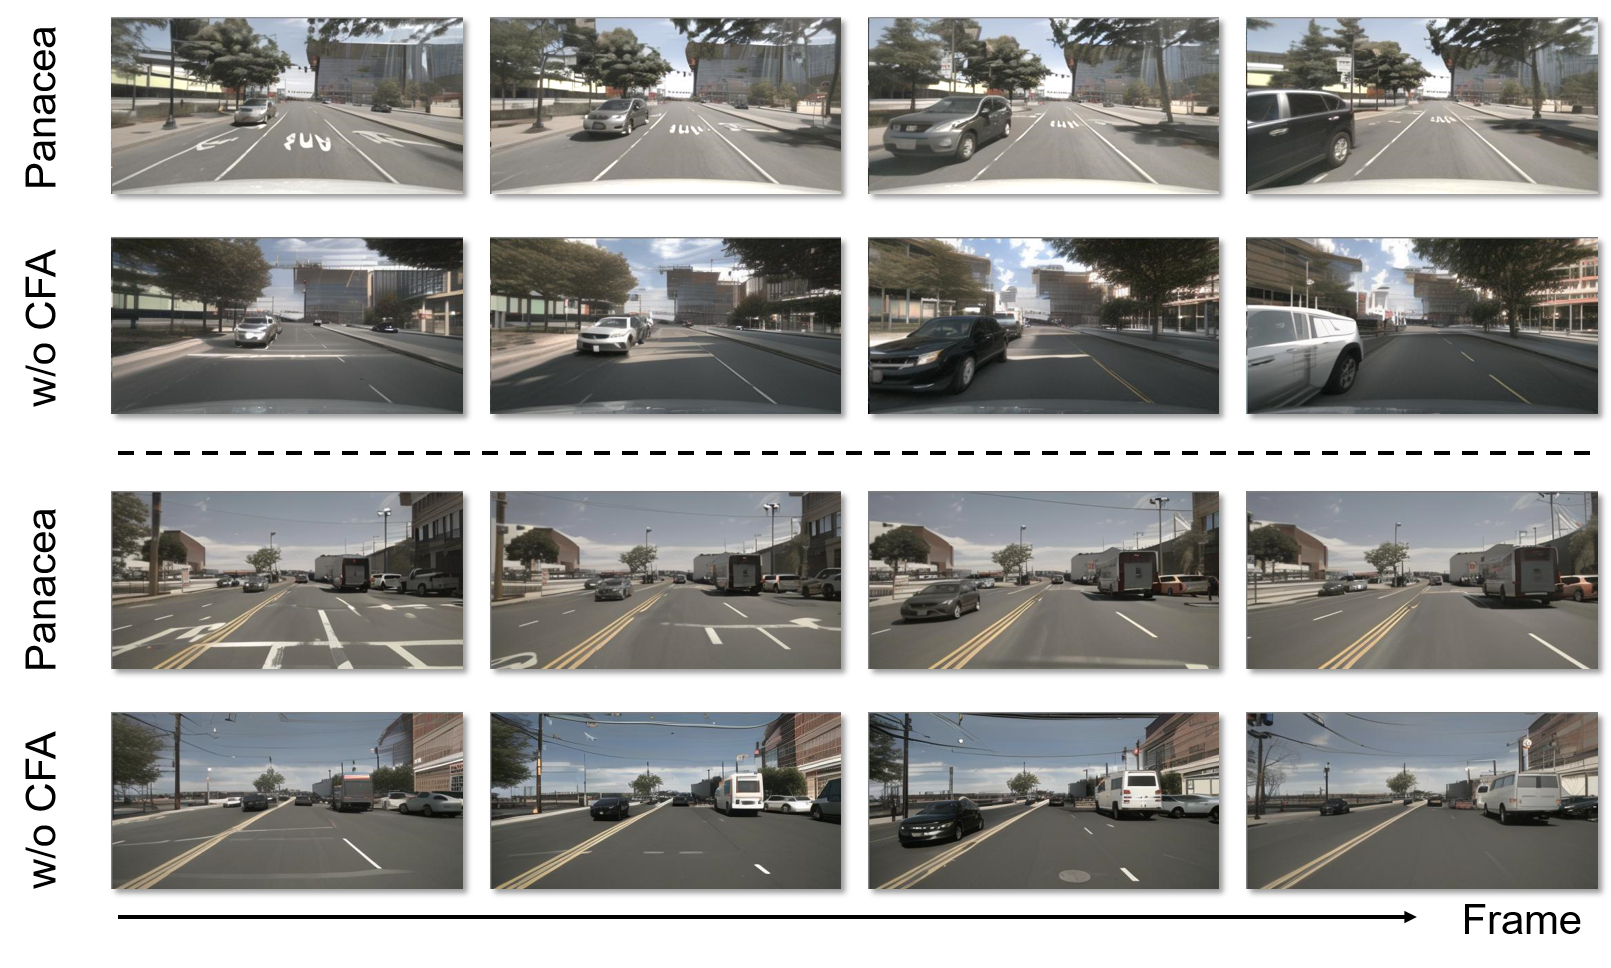
\includegraphics[width=0.5\linewidth]{figures/figure8.png}
% \caption{Samples of Identity Drift from Panacea's Paper (Fig.7, row 1):
% a car changes color from silver to black across frames.}
% \label{fig:panacea-paper}
% \vspace{-0.5cm}
% \end{figure}



\subsection{New Sample from Left-Hand for Non-Continuous Trajectory \textcolor{orange}{$@$R4-Q2/Q3}}

We thank the reviewer for the helpful suggestion. We have added a new example from the nuScenes validation set where a vehicle appears, disappears, and reappears in the Left-Front view. 
The qualitative result is shown in Fig.~\ref{fig:Non-Continuous2} (b), providing a more representative and higher-quality demonstration of our model’s ability to preserve instance identity under non-continuous trajectories.

We will add more representative and higher-quality results to showcase our method's capability on the Project Page.



\begin{figure}[ht]
\centering
\includegraphics[width=0.5\linewidth]{figures/continuous2.pdf}
\caption{Samples of Non-Continuous Trajectory generated by ConsisDrive with Instance-Masked Attention.
\textbf{(a)} In the Right-Front view, the black car is occluded and reappears while maintaining its identity.
\textbf{(b)} In the Left-Front view, the white car similarly preserves its appearance after occlusion and reappearance.}
\label{fig:Non-Continuous2}
%\vspace{-0.5cm}
\end{figure}

Thanks for your feedback again! It really helps me improve my manuscript to better showcase our research work!

Hope for your final review and final rating!

